\chapter{Análise de Valor} 
\label{chap:Chapter03} 

\section{Processo de Inovação}

\subsection{Conceito de Processo de Inovação}

O processo de inovação pode ser dividido em três áreas principais: o Fuzzy Front End (FFE), o Processo de Desenvolvimento de Novos Produtos (DNP) e a comercialização \parencite{BOOK01}. Cada uma dessas áreas desempenha um papel no ciclo de inovação, contribuindo para transformar ideias em produtos, serviços ou processos que geram valor para a organização e seus clientes. 

A primeira parte, Fuzzy Front End, é geralmente considerada uma das mais importantes para a melhoria do processo de inovação \parencite{BOOK01}. Essa fase inicial é caracterizada pela sua natureza incerta e exploratória, onde novas oportunidades de mercado são identificadas e um grande número de ideias é gerado e refinado.

Nesse capítulo, a atenção será voltada para as atividades do Fuzzy Front End, que têm objetivo de aumentar o valor, a quantidade e a probabilidade de sucesso dos conceitos lucrativos que entram nas fases posteriores de desenvolvimento e comercialização de produtos. Exploraremos práticas para identificar oportunidades promissoras, métodos eficazes para gerar e enriquecer ideias e estratégias para selecionar os conceitos mais viáveis.

\begin{figure}[h]
    \centering
    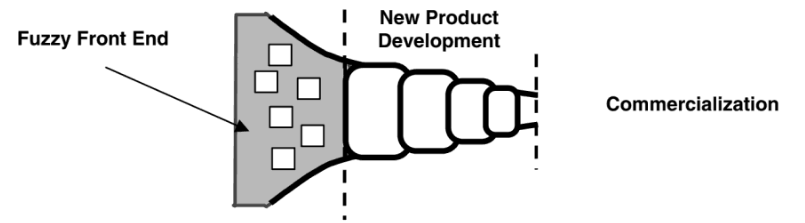
\includegraphics[scale=0.5]{ch03/assets/inovation-process.png}
    \decoRule
    \caption[Processo de Inovação]{Processo de Inovação \parencite{BOOK01}}
    \label{fig:ch02-inovation-process}
\end{figure}

\subsection{New Concept Development (NCD)}

O modelo \textit{New Concept Development} (NCD) é composto por três partes principais \parencite{BOOK01}:

\begin{itemize}
    \item \textbf{Parte central ou motor:} Consiste na liderança, cultura e estratégia de negócios da organização, que impulsionam os cinco elementos-chave controláveis pela empresa.
    
    \item \textbf{Área interna de raios:} Define os cinco elementos de atividade controláveis do Fuzzy Front End (FFE), que são: 
    \begin{itemize}
        \item Identificação de oportunidades
        \item Análise de oportunidades
        \item Geração e enriquecimento de ideias
        \item Seleção de ideias
        \item Definição de conceito
    \end{itemize}

    \item \textbf{Fatores de influência:} Incluem as capacidades organizacionais, o ambiente externo (como canais de distribuição, legislação, políticas governamentais, clientes, concorrentes e o clima político e econômico) e as ciências facilitadoras (tanto internas quanto externas). Esses fatores influenciam todo o processo de inovação até a comercialização e são relativamente incontroláveis pela empresa.
\end{itemize}

\begin{figure}[h]
    \centering
    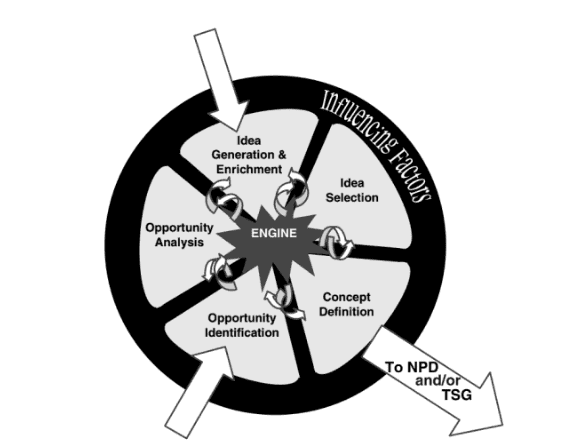
\includegraphics[scale=0.5]{ch03/assets/new-concept-development.png}
    \decoRule
    \caption[New Concept Development]{New Concept Development \parencite{BOOK01}}
    \label{fig:ch02-inovation-process}
\end{figure}

\subsection{Identificação da oportunidade}

Nessa atividade, se busca identificar oportunidades que possam ser exploradas para impulsionar o crescimento e eficiência \parencite{BOOK01}. Essa oportunidade pode representar uma nova direção para o negócio ou uma atualização de produtos existentes. Pode incluir o desenvolvimento de novas plataformas de produtos, processos de fabricação, ofertas de serviços ou abordagens de marketing e vendas. A identificação inicial da oportunidade define o mercado ou a área tecnológica na qual a solução irá se envolver.

A necessidade de desenvolver soluções acessíveis para o aprendizado do Braille é evidenciada pela alta demanda e os altos custos das Máquinas de escrever em Braille, como descrito em na seção \ref{sec:ch02_Valores_da_Maquina_Braille}. Pessoas com deficiência visual, especialmente aquelas que ficaram cegas recentemente, enfrentam barreiras significativas no acesso a essas ferramentas essenciais. Instituições educacionais e organizações dedicadas ao suporte de pessoas com deficiência visual também enfrentam desafios devido à necessidade de múltiplas máquinas para práticas em grupo. 

Portanto, a oportunidade reside em criar uma ferramenta virtual que possa preencher essa lacuna, proporcionando um ambiente de aprendizado eficaz e acessível.

\subsection{Análise da oportunidade}

Essa atividade envolve a identificação e avaliação de potenciais oportunidades de mercado, necessidades dos clientes, tendências tecnológicas e lacunas no mercado \parencite{BOOK01}. Nesta fase as informações podem ser incertas, ambíguas ou incompletas, o que significa que a análise de oportunidades pode ser desafiadora. A análise de oportunidades no Fuzzy Front End pode incluir técnicas como pesquisa de mercado, análise de tendências, brainstorming, análise SWOT (Strengths, Weaknesses, Opportunities, Threats), análise de cenários, entre outros métodos para identificar e entender as oportunidades que podem guiar o desenvolvimento de novos produtos ou serviços \parencite{BOOK01}. Nessa seção usaremos a técnica de análise SWOT.

Os principais beneficiários desta aplicação são pessoas com deficiência visual, educadores e instituições que oferecem suporte a essas pessoas. Esses usuários precisam de uma solução prática, acessível e eficaz para o aprendizado do Braille. A aplicação web deve ser intuitiva e replicar a experiência de usar uma Máquina de escrever em Braille, permitindo que os usuários pratiquem de forma realista. Além disso, deve oferecer feedback sonoro e visual para auxiliar no processo de aprendizado.

\begin{figure}[h]
    \centering
    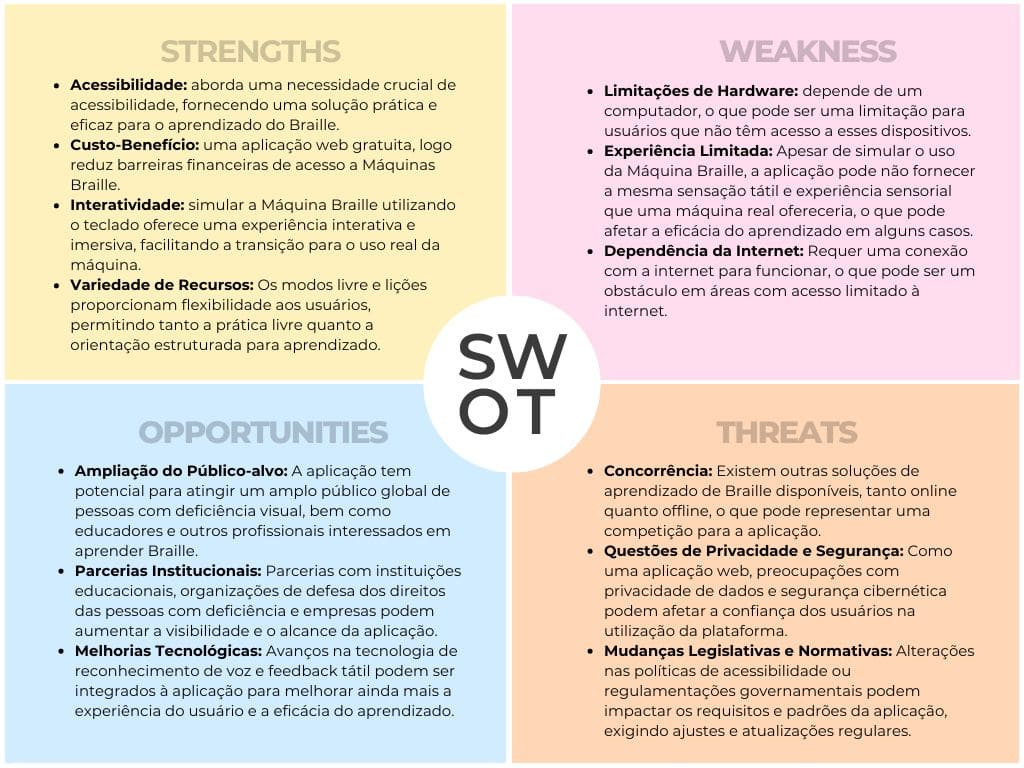
\includegraphics[scale=0.4]{ch03/assets/analise-swot.jpg}
    \decoRule
    \caption[Análise SWOT]{Análise SWOT}
    \label{fig:ch02-analise-swot}
\end{figure}

Inicialmente, as forças do projeto são notáveis. A acessibilidade é uma vantagem crucial, pois aborda uma necessidade significativa para pessoas com deficiência visual, fornecendo uma solução prática e gratuita para o aprendizado do Braille. Além disso, a interatividade oferecida pela aplicação, juntamente com sua variedade de recursos, como os modos de Modo Livre e Modo de Lições, promove uma experiência flexível e envolvente para os usuários.

No entanto, a aplicação possui algumas fraquezas a serem consideradas. A dependência do acesso a um computador pode excluir potenciais usuários que não têm acesso a esses dispositivos, enquanto a falta de sensação tátil pode limitar a experiência de aprendizado em comparação com o uso de uma máquina real. Além disso, a necessidade de uma conexão estável com a internet pode ser uma limitação em áreas com acesso limitado à rede.

Por outro lado, contém diversas oportunidades para ampliar seu impacto e alcance. Com potencial para atingir um amplo público global e estabelecer parcerias com instituições educacionais e organizações de defesa dos direitos das pessoas com deficiência, a aplicação pode expandir sua influência e utilidade. Além disso, a integração de melhorias tecnológicas, como reconhecimento de voz e feedback tátil, pode aprimorar ainda mais a experiência do usuário.

No entanto, o projeto também enfrenta ameaças, como a concorrência de outras soluções de aprendizado de Braille e preocupações com privacidade de dados e segurança cibernética. Mudanças nas políticas de acessibilidade ou regulamentações governamentais também podem representar desafios futuros que exigem adaptação e flexibilidade.

Em suma, embora o projeto apresente desafios significativos, suas forças e oportunidades superam essas limitações, o posicionando como uma ferramenta valiosa para promover a inclusão e a autonomia de pessoas com deficiência visual. Com uma abordagem estratégica e contínua inovação, o projeto tem o potencial de fazer uma diferença positiva na vida de muitos indivíduos.

\subsection{Geração e enriquecimento de ideias}

Nessas atividade é abordado o processo de concepção, desenvolvimento e refinamento de uma ideia concreta \parencite{BOOK01}. Esse processo é altamente iterativo e evolutivo, envolvendo a construção, destruição, combinação, remodelação, modificação e atualização de ideias. As ideias passam por diversas iterações e mudanças à medida que são exploradas, estudadas, discutidas e desenvolvidas em conjunto com outros elementos do modelo de Desenvolvimento de Novos Produtos \parencite{BOOK01}.

As principais funcionalidades da aplicação foram determinadas com base nas necessidades dos usuários:

\begin{itemize}
    \item \textbf{Simulação das teclas da Máquina Braille:} Utilização das teclas F, D, S, J, K e L para simular os pontos do Braille.
    \item \textbf{Feedback Sonoro:} Cada caractere escrito deve ser acompanhado por um feedback sonoro.
    \item \textbf{Modos de Uso:} Um Modo Livre para prática livre e um Modo de Lições com exercícios estruturados.
    \item \textbf{Visualização do Texto}: Exibição do texto em Braille e em tinta para facilitar o entendimento dos usuários.
    \item \textbf{Navegação:} Uso das setas do teclado para navegar pelo texto.
\end{itemize}

\subsection{Seleção da ideia}

A seleção de ideias envolve uma série iterativa de atividades, que incluem múltiplas revisões da identificação de oportunidades, análise de oportunidades e geração e enriquecimento de ideias \parencite{BOOK01}. 

Durante a fase de geração de ideias, diversas propostas foram consideradas para o desenvolvimento da aplicação simuladora da Máquina de escrever em Braille. Cada ideia foi avaliada com base em sua capacidade de atender às necessidades dos usuários e oferecer uma solução acessível, prática e eficaz para o aprendizado e prática do Braille. Após análise, todas as ideias foram selecionadas para compor o conceito final da aplicação.

Cada uma dessas ideias foi considerada crucial para o desenvolvimento de uma aplicação web simuladora da Máquina de escrever em Braille que seja acessível, prática e eficaz. A combinação dessas funcionalidades proporcionará uma experiência completa e satisfatória para os usuários, contribuindo assim para a promoção da inclusão e autonomia de pessoas com deficiência visual.

\subsection{Definição do conceito}

A definição do conceito é a última atividade no novo modelo de desenvolvimento de produtos. Nesse estágio, o inovador precisa convencer os responsáveis pela decisão a investirem na proposta de negócio ou tecnologia. Isso é muitas vezes chamado de "declaração de vitória" ou "documento de entrada". Geralmente, são considerados objetivos, tamanho da oportunidade ou até mesmo necessidades do mercado ou do cliente \parencite{BOOK01}.

O conceito para a aplicação foi definido para atender às necessidades dos usuários e proporcionar uma solução acessível, prática e eficaz para o aprendizado e prática do Braille. Através da análise das ideias geradas e da seleção das funcionalidades mais relevantes, o conceito final da aplicação é por vários pontos.

\subsubsection{Simulação Precisa da Máquina Braille}

A aplicação irá mapear as teclas do teclado do computador para simular os pontos do Braille, garantindo uma representação fiel da Máquina Braille real. Cada tecla correspondente aos pontos do Braille será atribuída a uma tecla específica do teclado, proporcionando uma experiência autêntica para os usuários.

\subsubsection{Feedback Multissensorial}

Será fornecido feedback sonoro e visual para cada caractere digitado. Quando uma tecla for pressionada, um som específico será reproduzido, indicando o caractere correspondente. Além disso, o caractere será exibido na tela em formato Braille, permitindo que os usuários visualizem o resultado de sua entrada.

\subsubsection{Modos de Uso Versáteis}

A aplicação oferecerá diferentes modos de uso para atender às necessidades dos usuários. No Modo Livre, os usuários podem praticar livremente, digitando textos e explorando a funcionalidade da Máquina Braille. No Modo de Lições, serão disponibilizados exercícios estruturados para facilitar o aprendizado do Braille, guiando os usuários por meio de atividades interativas.

\subsubsection{Visualização do Texto em Braille e em Tinta}

O texto digitado será apresentado tanto em Braille quanto em tinta, permitindo que os usuários visualizem o conteúdo de forma acessível. Essa funcionalidade visa atender às necessidades de usuários menos familiarizados com o Braille, facilitando sua compreensão do texto.


\section{Valor da solução}

\subsection{Valor}

O conceito de valor, especialmente no contexto de marketing, é essencial para entender a lealdade e satisfação do cliente \parencite{BOOK02}. Diversos autores ofereceram definições e perspectivas distintas sobre o que constitui valor. \textcite{BOOK03} define valor como uma crença duradoura na preferência por um modo de conduta ou estado final específico em detrimento de outro. \textcite{ARTICLE10}, por sua vez, apresenta três definições: valor como preço baixo, como a qualidade recebida pelo preço pago e como o trade-off entre o que se recebe e o que se dá. Esta última definição é complementada por \textcite{BOOK04}, que também destacam o trade-off entre a qualidade do item e seus custos.

Desenvolvendo ainda mais a noção de trade-off, \textcite{BOOK05} define valor como a diferença entre os benefícios percebidos e os sacrifícios percebidos pelos clientes. Benefícios percebidos podem incluir qualidade do produto, serviço associado, benefícios relacionais e de imagem, enquanto os sacrifícios incluem custos monetários, de tempo, energia e psicológicos. \textcite{BOOK06} ampliam essa definição, considerando o valor como a soma dos benefícios técnicos, econômicos, de serviço e sociais que um cliente recebe em troca do preço pago. Esta abordagem destaca que o valor é uma avaliação subjetiva do cliente, baseada na percepção dos benefícios recebidos em comparação com os custos incorridos.

Finalmente, é importante reconhecer que o conceito de valor pode variar conforme a perspectiva do cliente. \textcite{ARTICLE11} observa que as percepções de “o que é recebido” e “o que é dado” variam de cliente para cliente, enfatizando que o valor é um trade-off entre esses componentes. Em termos práticos, muitas vezes os proprietários de negócios, resumem valor na simples máxima "você recebe o que paga", refletindo a inter-relação entre preço, qualidade e satisfação do cliente. Assim, compreender o valor de maneira holística e adaptada às percepções dos clientes é crucial para as estratégias de marketing e fidelização.

\subsection{Valor do produto}

\textcite{ARTICLE10} afirma que o conceito de valor do produto para o cliente (\textit{perceived value}) varia entre os consumidores, refletindo suas percepções pessoais. Entrevistados utilizam o termo "valor" de maneiras diversas, abrangendo uma ampla gama de atributos e abstrações. Esse valor é altamente subjetivo e pode ser definido de quatro formas principais: 

\begin{enumerate}
    \item \textbf{Valor é preço baixo}, onde o custo é o fator predominante;
    \item \textbf{Valor é tudo o que quero em um produto}, enfatizando a satisfação dos desejos e utilidades individuais;
    \item \textbf{Valor é a qualidade que obtenho pelo preço que pago}, onde a troca justa entre preço e qualidade é crucial;
    \item \textbf{Valor é o que recebo pelo o que dou}, considerando um equilíbrio entre todos os benefícios recebidos e os custos suportados.
\end{enumerate}

Essas definições demonstram a complexidade de conceituar e medir o valor percebido na pesquisa de marketing. Enquanto alguns consumidores focam principalmente no aspecto monetário, outros dão mais importância aos benefícios e conveniências que o produto oferece. Há também aqueles que veem valor como uma troca equilibrada entre preço e qualidade, e outros que consideram todos os aspectos de dar e receber na sua avaliação de valor \parencite{ARTICLE10}.

Segundo \textcite{ARTICLE10}, a perspectiva longitudinal do valor do produto para o cliente pode ser segmentada em quatro fases principais: 

\begin{itemize}
    \item Antes da compra;
    \item Na aquisição;
    \item Após a compra;
    \item Após o uso ou experiência.
\end{itemize}

No estágio pré-compra, o valor é percebido através do "valor desejado" e "valor esperado", onde os clientes formam expectativas sobre os benefícios que esperam obter e os sacrifícios que estão dispostos a fazer \parencite{ARTICLE10}. Durante a aquisição, o valor é experimentado em tempo real como "valor de transação" e "valor de aquisição", refletindo a avaliação imediata dos benefícios recebidos contra os sacrifícios feitos, como o custo e o esforço da compra \parencite{ARTICLE10}. Após a compra, o valor se manifesta como "valor entregue", "valor recebido', "valor de uso' e "valor pós-compra/desempenho", onde os clientes avaliam os benefícios contínuos e a utilidade do produto ou serviço, considerando os sacrifícios já realizados \parencite{ARTICLE10}. Finalmente, após o uso ou experiência, o valor é percebido como "valor de resgate", considerando os benefícios remanescentes ou o valor residual no ponto de disposição ou revenda, contrastando com os sacrifícios iniciais e contínuos feitos \parencite{ARTICLE10}. 

\begin{figure}[h]
    \centering
    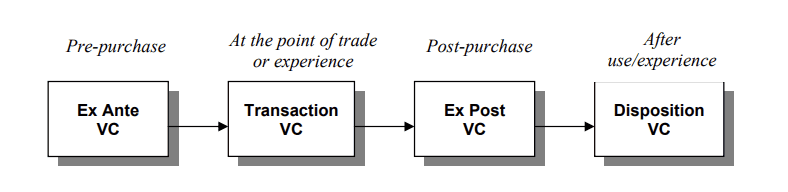
\includegraphics[scale=0.7]{ch03/assets/longitudinal-perspective.png}
    \decoRule
    \caption[Perspectiva longitudinal do valor do produto para o cliente]{Perspectiva longitudinal do valor do produto para o cliente \parencite{ARTICLE10}}
    \label{fig:ch02-longitudinal-perspective}
\end{figure}

Essa estrutura longitudinal revela como o valor do produto para o cliente evolui ao longo do tempo, influenciando as percepções de benefícios e sacrifícios dos clientes em diferentes etapas de sua jornada.

\subsubsection{Antes da Compra}

\textbf{Benefícios:}

\begin{itemize}
    \item \textbf{Acessibilidade:} A aplicação web é gratuita e disponível online, eliminando a barreira financeira que impede o acesso às máquinas Braille físicas.
    \item \textbf{Praticidade:} Permite o aprendizado e prática do Braille em qualquer lugar com acesso a um computador, sem a necessidade de equipamento especializado.
    \item \textbf{Inclusão:} Oferece uma solução inclusiva que pode ser usada por pessoas recém-deficientes visuais e por educadores em ambientes de ensino inclusivo.
\end{itemize}

\textbf{Sacrifícios:}

\begin{itemize}
    \item \textbf{Necessidade de Recursos:} O usuário precisa ter acesso a um computador com teclado físico e conexão à internet.
    \item \textbf{Curva de Aprendizado Inicial:} Usuários que não estão familiarizados com o uso de computadores podem encontrar dificuldades iniciais.
\end{itemize}

\subsubsection{Na Aquisição}

\textbf{Benefícios:}

\begin{itemize}
    \item \textbf{Imediata Disponibilidade:} A aplicação pode ser acessada e utilizada instantaneamente após a obtenção do link ou acesso à plataforma.
    \item \textbf{Custo Zero:} Não há custo financeiro envolvido na aquisição, tornando a solução extremamente acessível.
\end{itemize}

\textbf{Sacrifícios:}

\begin{itemize}
    \item \textbf{Dependência Tecnológica:} Requer conhecimentos básicos de navegação na web e uso de teclados de computador, o que pode ser um obstáculo para alguns usuários.
    \item \textbf{Configuração Inicial:} Pode ser necessário ajustar configurações do navegador ou do computador para otimizar o uso da aplicação (por exemplo, desativar teclas de atalho conflitantes).
\end{itemize}

\subsubsection{Após a Aquisição}

\textbf{Benefícios:}

\begin{itemize}
    \item \textbf{Feedback Imediato:} A aplicação fornece feedback sonoro imediato sobre os caracteres digitados, ajudando no aprendizado rápido e na correção de erros.
    \item \textbf{Modo de Lições:} O modo de lições oferece exercícios estruturados, facilitando o aprendizado sistemático do Braille.
    \item \textbf{Versatilidade:} A capacidade de visualizar textos tanto em Braille quanto em texto regular facilita o aprendizado e a correção por parte de educadores e familiares.
\end{itemize}

\textbf{Sacrifícios:}

\begin{itemize}
    \item \textbf{Dependência de Dispositivos:} O usuário ainda precisa de um computador e, eventualmente, de dispositivos de som para maximizar o uso da aplicação.
    \item \textbf{Possíveis Dificuldades Técnicas:} Problemas técnicos relacionados à aplicação ou ao hardware do usuário podem surgir, necessitando de resolução.
\end{itemize}

\subsubsection{Após a Utilização}

\textbf{Benefícios:}

\begin{itemize}
    \item \textbf{Autonomia e Independência:} A prática contínua com a aplicação promove a autonomia dos usuários, preparando-os para o uso de máquinas Braille físicas.
    \item \textbf{Transição Facilitada:} A experiência adquirida com o simulador facilita a transição para o uso real da máquina de escrever em Braille.
    \item \textbf{Inclusão Social:} Contribui para a inclusão social e profissional das pessoas com deficiência visual, permitindo-lhes participar plenamente de atividades que requerem leitura e escrita em Braille.
\end{itemize}

\textbf{Sacrifícios:}

\begin{itemize}
    \item \textbf{Continuidade do Suporte:} Para manter a eficácia da ferramenta, pode haver a necessidade de suporte contínuo ou atualizações da aplicação.
    \item \textbf{Limitações de Simulação:} A experiência virtual, apesar de eficaz, pode não reproduzir perfeitamente todas as nuances do uso de uma máquina Braille física.
\end{itemize}

A aplicação oferece um valor significativo antes da compra, na aquisição, após a aquisição e após a utilização. Os benefícios incluem acessibilidade, imediata disponibilidade, feedback educativo e promoção da autonomia, enquanto os sacrifícios envolvem a necessidade de recursos tecnológicos e possíveis dificuldades técnicas. No geral, a aplicação representa uma solução valiosa e prática para a inclusão e capacitação de pessoas com deficiência visual.

\subsection{Proposta de valor}

Segundo \textcite{ARTICLE12}, a proposta de valor é uma ferramenta estratégica que facilita a comunicação de uma organização em compartilhar recursos e oferecer um pacote de valor superior aos clientes-alvo. Essa definição destaca a importância da proposta de valor como um meio essencial para as empresas demonstrarem como seus produtos ou serviços se destacam no mercado, proporcionando benefícios únicos e diferenciados. Ao comunicar claramente essa proposta, as organizações conseguem atrair e reter clientes, mostrando de forma convincente as vantagens e valores que podem oferecer em comparação com seus concorrentes.

\begin{figure}[h]
    \centering
    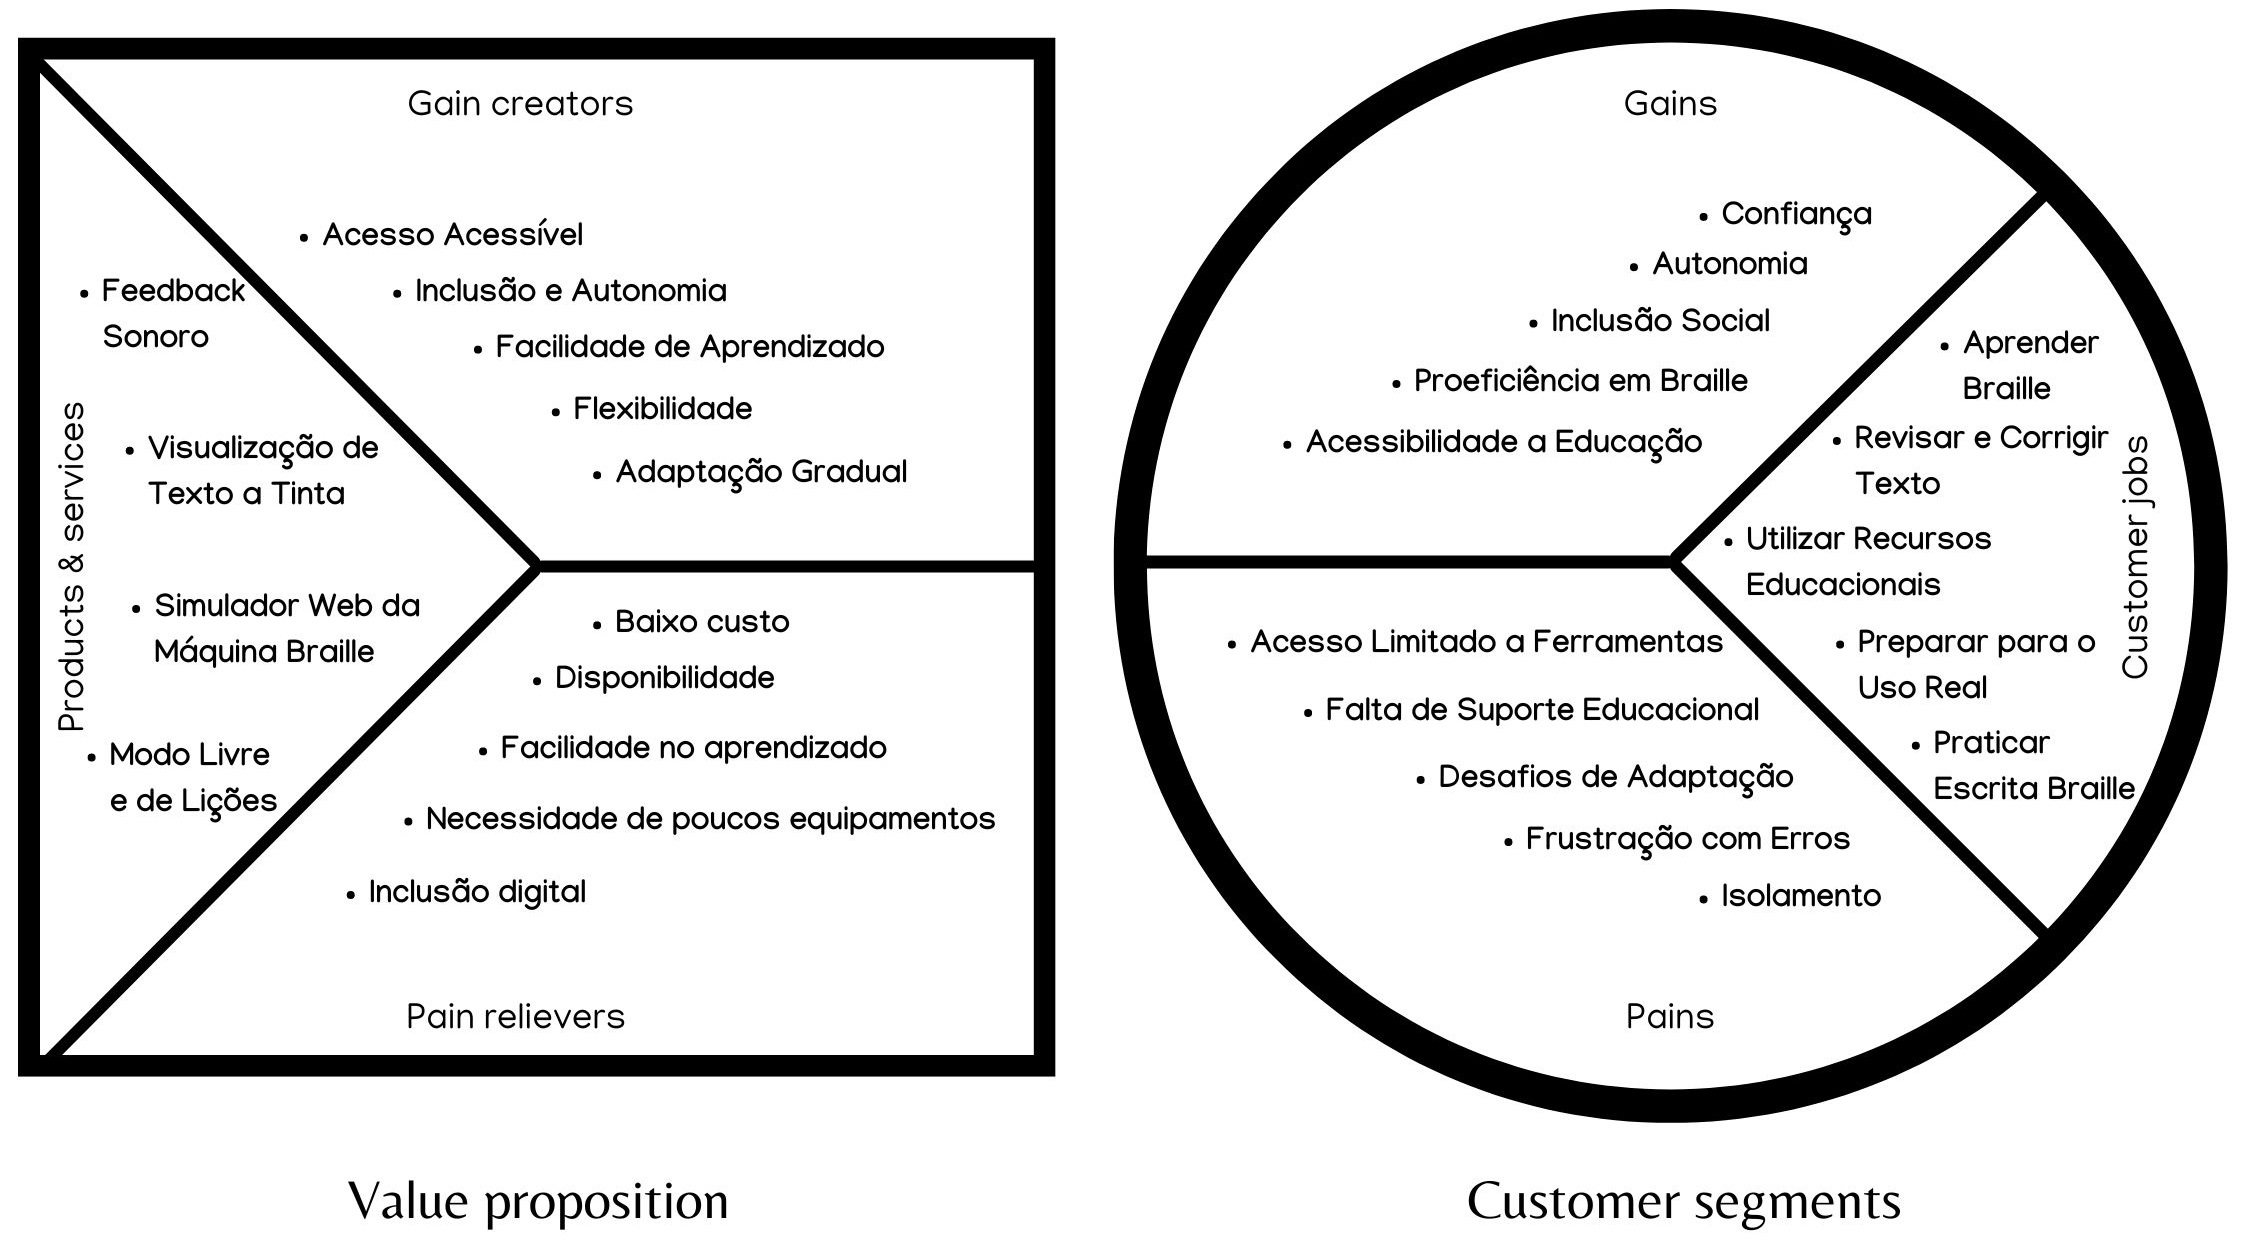
\includegraphics[scale=0.15]{ch03/assets/value-proposition.jpg}
    \decoRule
    \caption[Proposta de valor]{Proposta de valor}
    \label{fig:ch02-longitudinal-perspective}
\end{figure}

\subsubsection{Tarefas do Cliente}

Os clientes da aplicação têm como principal tarefa aprender a ler e escrever em Braille de maneira eficiente. Eles precisam praticar regularmente para ganhar fluência e confiança na escrita Braille. Outra tarefa importante é se preparar para o uso de uma Máquina Braille física, ganhando familiaridade com a disposição das teclas e os padrões de escrita. A revisão e correção do texto escrito são facilitadas pela navegação com as setas do teclado, melhorando a precisão e a qualidade da escrita. Além disso, os clientes utilizam os recursos educacionais fornecidos pela aplicação, aproveitando as lições e exercícios estruturados para aprimorar seu conhecimento e habilidade em Braille.

\subsubsection{Ganhos}

Com o uso da aplicação, os clientes aumentam significativamente sua proficiência em ler e escrever em Braille. Essa habilidade promove maior autonomia, permitindo que se comuniquem de forma independente utilizando Braille. A inclusão social é outro ganho importante, pois os usuários podem participar plenamente de atividades educacionais e profissionais que requerem o uso do Braille. 

A autoconfiança dos usuários também aumenta à medida que se tornam mais competentes na escrita Braille. Além disso, a aplicação oferece acesso a materiais educativos e oportunidades de aprendizado sem a necessidade de equipamentos caros, facilitando a educação contínua em Braille.

\subsubsection{Dores}

Antes da existência da aplicação, muitos enfrentavam acesso limitado a ferramentas de aprendizado de Braille devido ao alto custo das Máquinas Braille. A falta de suporte educacional adequado também é um problema significativo, dificultando o aprendizado de Braille. Cometer erros frequentes na escrita em Braille sem um sistema de correção acessível causa frustração, e o sentimento de isolamento é comum entre aqueles que não podiam participar plenamente de atividades que requerem o conhecimento do Braille.

\subsubsection{Produtos e Serviços}

A aplicação oferece uma interface interativa que permite aos usuários praticarem a escrita Braille usando o teclado do computador. Com dois modos de operação distintos, o Modo Livre permite a prática livre, onde os usuários podem escrever e visualizar o texto em células Braille sem restrições. O Modo de Lições oferece uma série de exercícios e lições estruturadas para facilitar o aprendizado do sistema Braille e o uso da Máquina Braille. 

Adicionalmente, a aplicação inclui uma funcionalidade que traduz o texto Braille para texto a tinta, tornando-o legível para aqueles que não estão familiarizados com Braille. Para aprimorar a experiência de aprendizado, a aplicação fornece feedback sonoro indicando qual caractere foi escrito, e permite a navegação pelo texto usando as setas do teclado, facilitando a revisão e correção do texto.

\subsubsection{Criadores de Ganho}

A aplicação é acessível ao aprendizado de Braille, pois elimina os custos associados à compra de uma Máquina Braille física. Ao oferecer uma ferramenta prática e gratuita, promove a inclusão e autonomia das pessoas com deficiência visual, permitindo que pratiquem de forma independente. A estrutura de lições e exercícios facilita o aprendizado, tornando-o mais eficiente e interativo. A flexibilidade de poder praticar a qualquer hora e em qualquer lugar, sem a necessidade de equipamento especializado, é uma grande vantagem. Além disso, a aplicação prepara gradualmente o usuário para a transição ao uso de uma Máquina Braille real, tornando o processo menos intimidante e mais confortável.

\subsubsection{Alívio das Dores}

A aplicação elimina a barreira do custo elevado das Máquinas Braille físicas, tornando o aprendizado de Braille mais acessível. Ao fornecer um recurso facilmente acessível e disponível online, resolve a falta de recursos adequados para o aprendizado de Braille. A interface amigável e o feedback contínuo simplificam o processo de aprendizagem, aliviando a dificuldade associada ao aprendizado de um novo sistema de escrita. 

Para ambientes educacionais, a aplicação remove a necessidade de múltiplas Máquinas Braille físicas, permitindo práticas em grupo de forma virtual e inclusiva. Finalmente, ao oferecer uma solução tecnológica moderna, a aplicação promove a inclusão digital, permitindo que qualquer pessoa com um computador e teclado possa aprender Braille.

\section{Valor para o cliente}

O Canvas Business Model é uma ferramenta estratégica desenvolvida por Alexander Osterwalder e Yves Pigneur, projetada para ajudar empresas a delinear, visualizar e inovar seus modelos de negócio. O Canvas Business Model se tornou amplamente utilizado tanto na academia quanto na prática empresarial. 

A ferramenta divide um modelo de negócio em nove blocos principais: segmentos de clientes, proposição de valor, canais, relacionamento com clientes, fontes de receita, recursos-chave, atividades-chave, parcerias-chave e estrutura de custos. Essa divisão incentiva os empreendedores a analisar cada elemento do negócio de forma detalhada e integrada, promovendo a reflexão constante, criatividade e inovação. 

Esta seção aborda o valor da aplicação para o cliente de forma mais profunda, utilizando a estrutura do Canvas Business Model. Essa análise  é crucial para entender como a aplicação atenderá às necessidades de seus usuários, promovendo a inclusão e autonomia de pessoas com deficiência visual.


\begin{figure}[h]
    \centering
    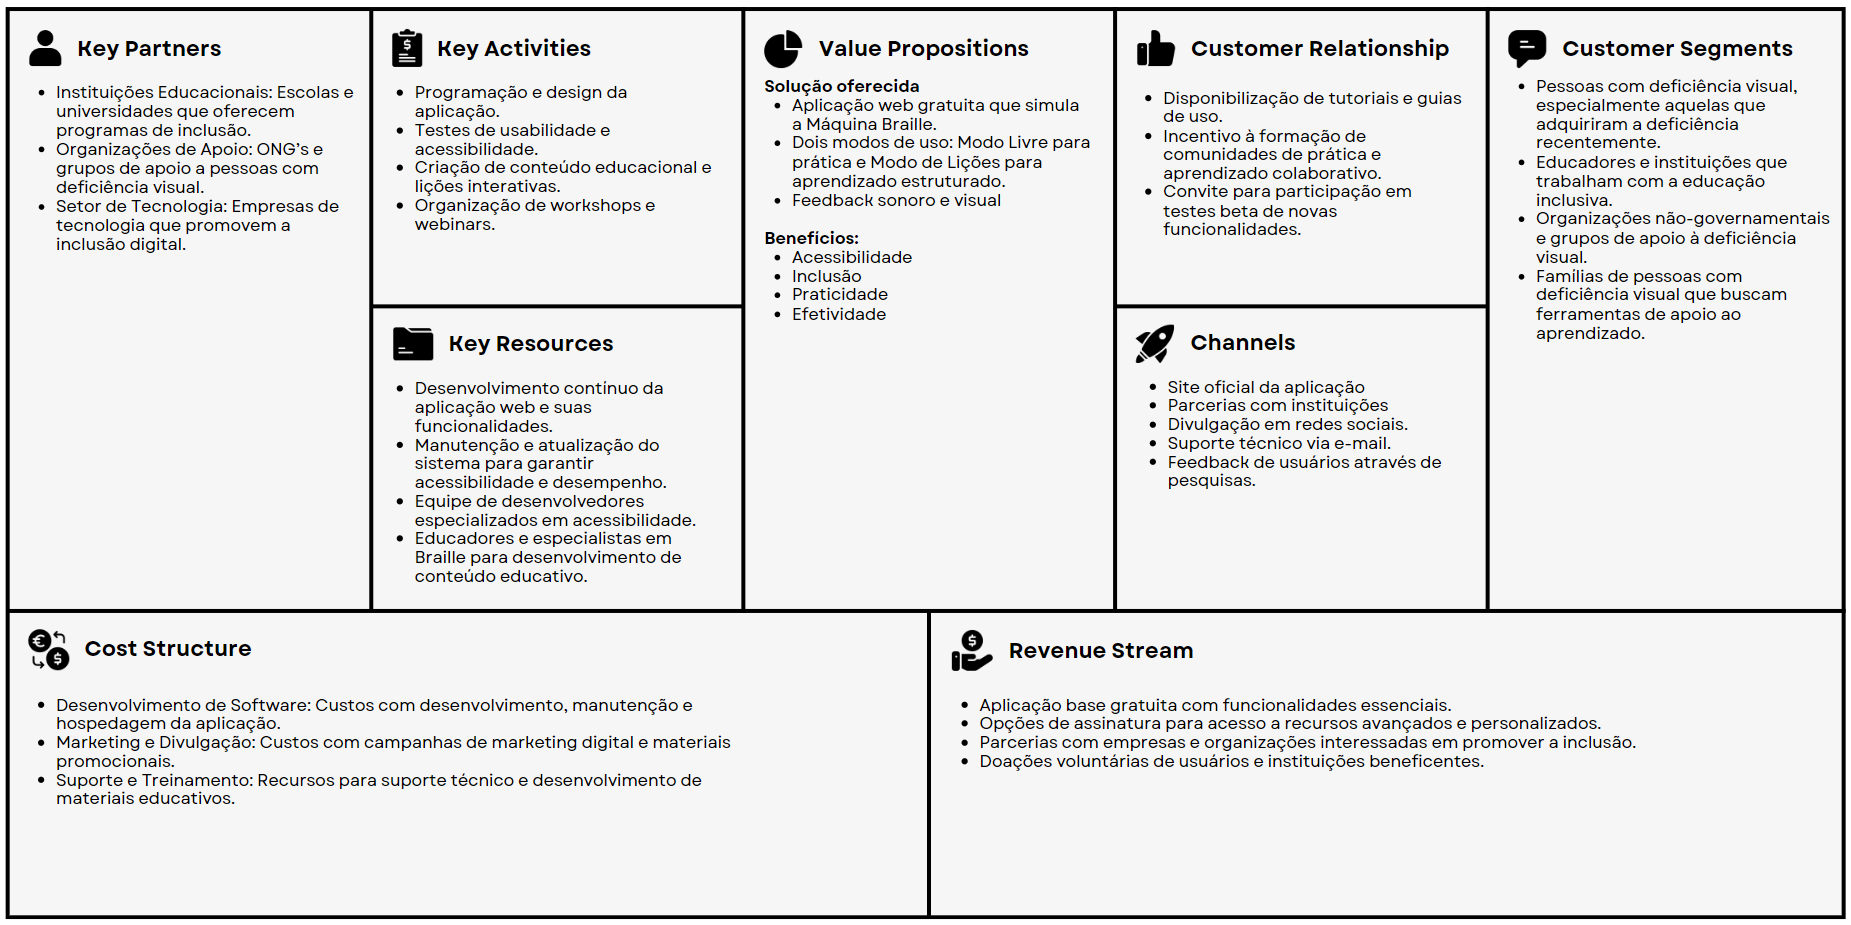
\includegraphics[scale=0.3]{ch03/assets/canva-business-model.png}
    \decoRule
    \caption[Canvas Business Model]{Canvas Business Model}
    \label{fig:ch02-canva-business-model}
\end{figure}

\section{Sumário}

Esta capítulo detalhou o valor da aplicação Web simuladora da Máquina de Escrever em Braille. A aplicação oferece uma solução prática, acessível e inclusiva, promovendo a autonomia de pessoas com deficiência visual e facilitando o aprendizado do Braille de maneira eficaz.


